\documentclass[../main.tex]{subfile}

\begin{document}

\section{Le rêve insinué}

La base même d'un rêve est les sensations qu'il produit pour le sujet. Ces
sensations sont au-délà des simples informations sur le monde extérieur
auquelles nous sommes habitués. Elles présentes certaines caractéristiques qui
sont intéressantes à reproduire pour imiter cet effet.

Généralement, un rêve est accompagné d'un état inconscient (sauf dans le cas
d'un \emph{rêve lucide}). C'est le premier outil à disposition du réalisateur :
si le spectateur ne sait pas qu'il observe un rêve, l'effet est accru au moment
où il s'en rend compte.

Cependant, cette idée est bien plus difficile à réaliser qu'il n'y paraît. Un
spectateur n'a a sa disposition que \emph{la vue} et \emph{l'ouïe} comme canaux
de communication avec l'univers du film regardé. Pourtant, au sein d'un rêve,
le sujet perçoit une grande variété de sensations différentes. C'est donc un
problème majeur pour la reproduction d'un rêve dans une \oe{}uvre
cinématographique.

\subsection{Aspect visuel}

Le cinéma est avant tout un \textbf{art photographique}, et à l'origine n'était
qu'une projection d'images sensées reproduire une histoire pour le spectateur.

La représentation visuelle d'un rêve est cruciale car c'est le moyen de
dialogue privilégié entre le réalisateur et le spectateur.

\subsubsection{Lenteur des images}

Pour simuler l'état d'inconscience accompagnant le rêve, le spectateur est
souvent entraîné dans une hypnose partielle, notamment à travers une lenteur
exagérée des images.

On peut voir par exemple dans \textit{Lost Highway (1997)} (figure
\ref{fig:images_long}), des longs plans centrés sur la route, qui semble se
dérouler à l'infini devant nous.

Pour le spectateur assis confortablement depuis un certain temps dans une salle
sombre, souvent avec une musique douce et pesante, l'effet est net.

\begin{figure}
    \centering
    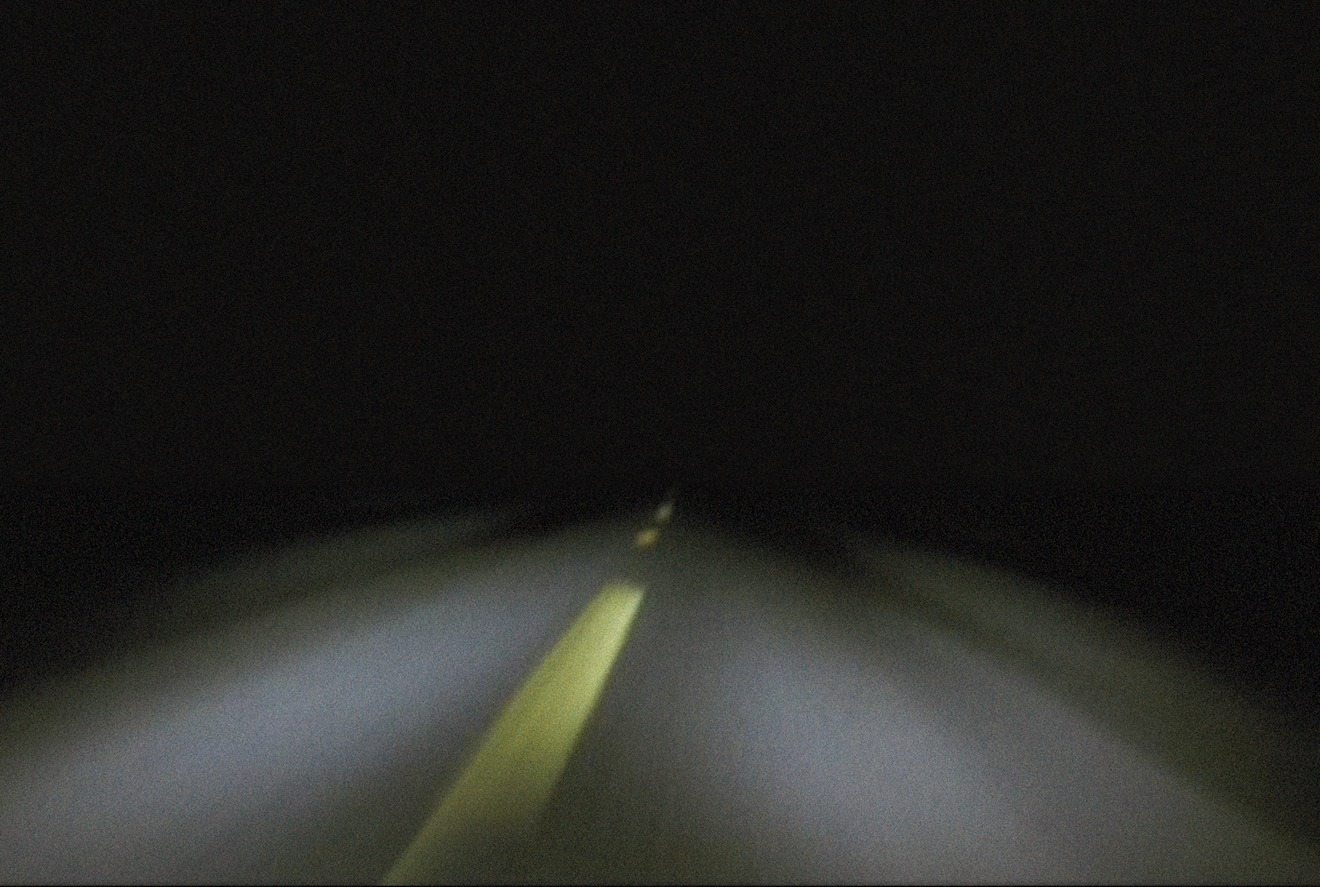
\includegraphics[width=\linewidth]{images/long}
    \caption{Lenteur photographique, \textit{Lost Highway (1997)}, un film de David Lynch}
    \label{fig:images_long}
\end{figure}

\subsubsection{Abondance de couleurs}

Une technique de représentation est l'utilisation excessive de
\textbf{contrastes de couleurs}. Cette méthode a l'avantage de captiver le
regard du spectateur sans pour autant trop en dire sur l'environnement.

En effet, le cinéma étant un art photographique, le spectateur peut confondre
la vision imposée par le réalisateur avec celle perçue par le(s) personnage(s)
dans le film.

\begin{figure}
    \centering
    
\includegraphics[width=\linewidth]{images/colors}
    \caption{Abondance de couleurs, \textit{Waking Life (2001)}}
    \label{fig:images_colors}
\end{figure}

Dans \textit{Waking Life (2001)} (figure \ref{fig:images_colors}), l'intégralité
du film est un rêve, presque une excuse pour pouvoir produire un film
entièrement par \textbf{animation rotoscopique}. Cette méthode consiste à
redessiner chaque image filmée pour mêler réalité et fiction, très adaptée à
l'exploration du monde onirique.

\subsubsection{Troubles visuels}

Le rêve est souvent décrit comme \emph{confus}, parfois \emph{clair} mais le
plus souvent \emph{instable}. Une reproduction visuelle de ces constatations
est bien difficile et risque, dans le pire des cas, de perdre l'attention du
spectateur. Alors comment montrer des images troubles, tout en maintenant
l'attention du spectateur ?

Cette technique est peu utilisée au vu des difficultés l'accompagnant, mais
certains réalisateurs ont tenté de l'utiliser. Un des plus remarquables reste
\textit{Inland Empire (2006)} de David Lynch (figure \ref{fig:images_trouble}),
scène dans laquelle le personnage principal sombre dans un état de
\emph{limbo}. Un flou a été forcé sur l'image à l'édition, intégrant une
brûlure de cigarette sur le mur (un élément important dans le rêve du
personnage). Il s'agit ici d'un trouble photographique ne reflétant pas
forcément le point de vue du personnage, mais celui qui est imposé sur le
spectateur.

Dans le cas de \textit{Waking Life (2001)} (figure \ref{fig:images_trouble2}),
les éléments du rêve ont été déformés sans déformer la vision du spectateur,
montrant le point de vue du personnage.

\begin{figure}
    \centering
    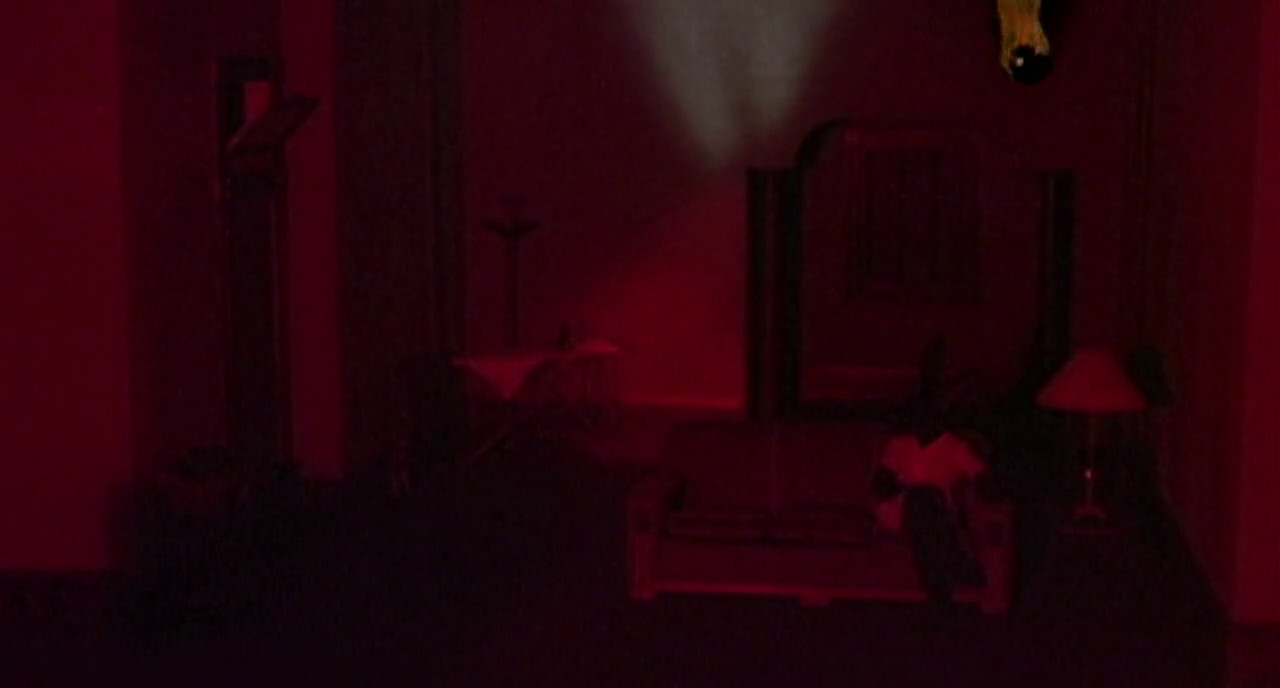
\includegraphics[width=\linewidth]{images/trouble}
    \caption{Trouble photographique, \emph{Inland Empire (2006)}}
    \label{fig:images_trouble}
\end{figure}

\begin{figure}
    \centering
    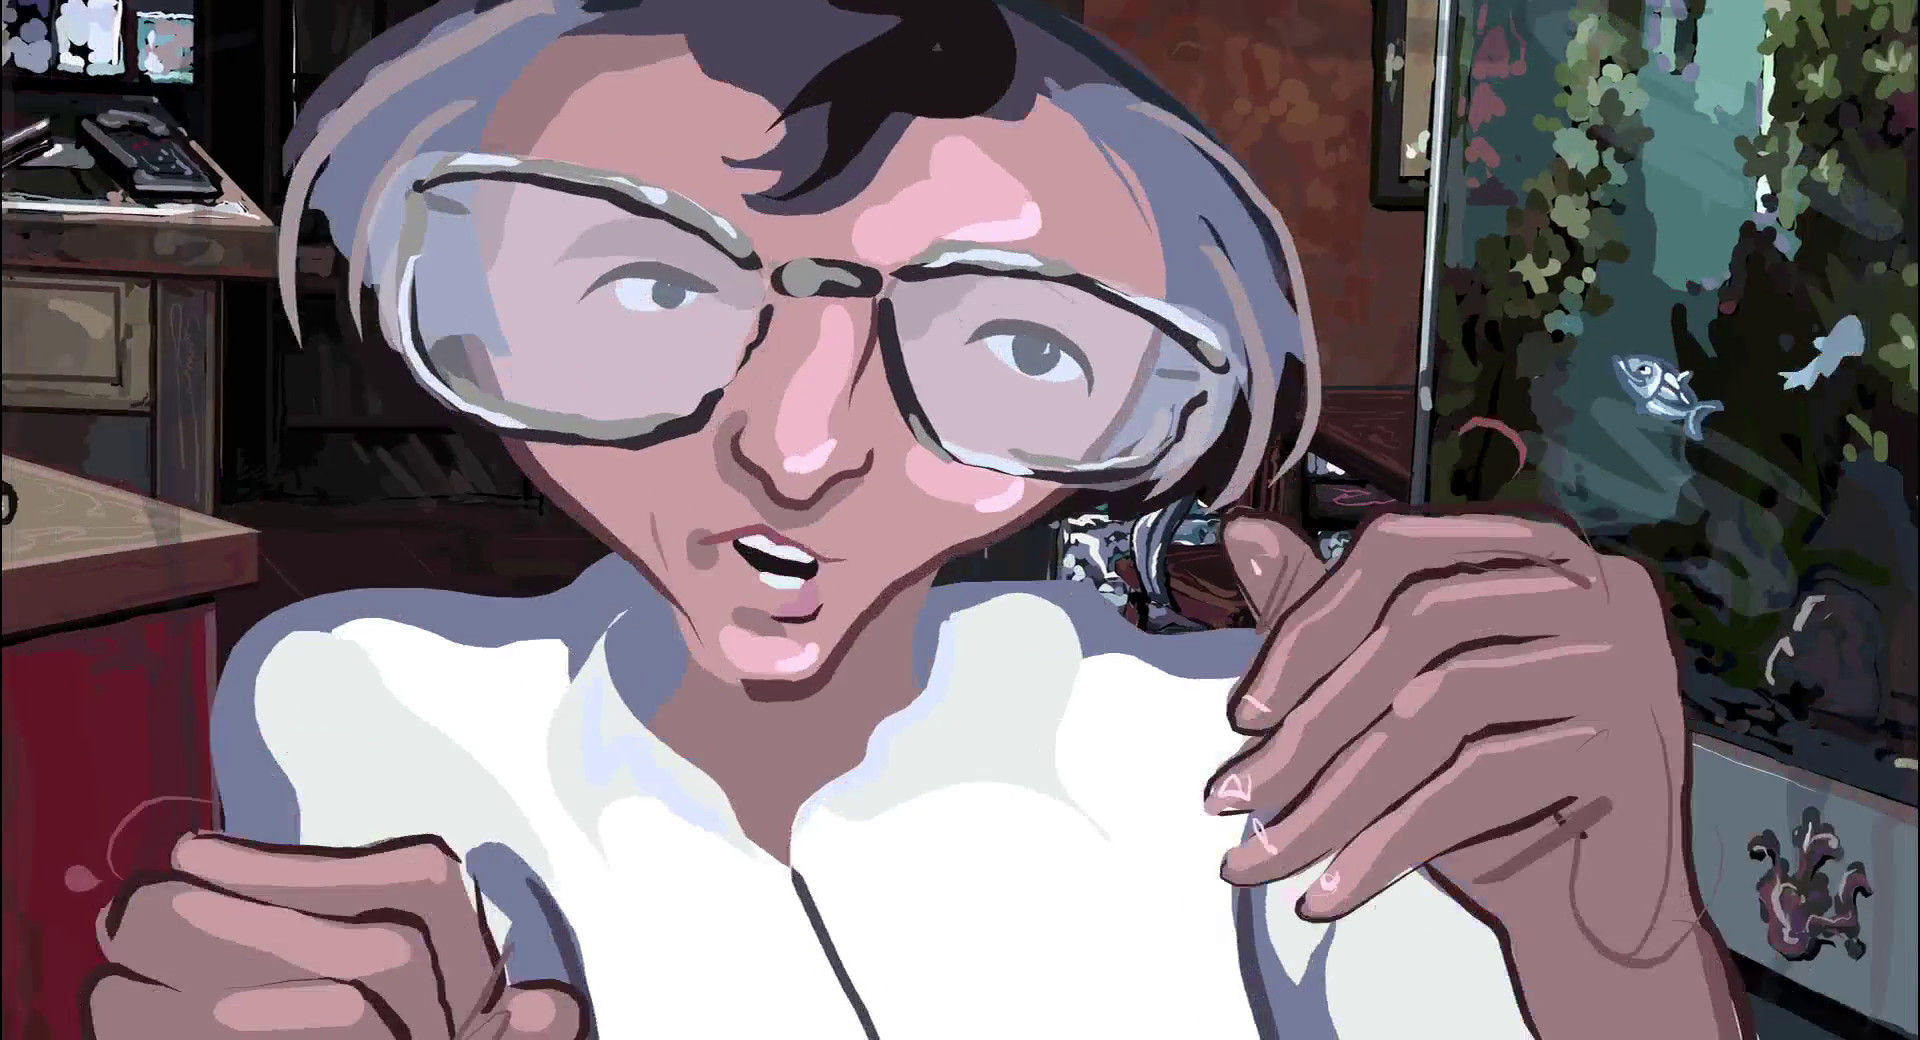
\includegraphics[width=\linewidth]{images/trouble2}
    \caption{Troubles visuels du personnage, \emph{Waking Life (2001)}}
    \label{fig:images_trouble2}
\end{figure}

\subsection{Aspect auditif}

\subsection{Symbolisme}

\end{document}
